\chapter{The nucleon-nucleon potential}

Since Chadwick discovered the neutron in 1932, understanding the 
nucleon-nucleon interaction has been a main focus for nuclear physicists.
Yukawa \cite{yukawa35} proposed the first significant theory of the nuclear 
force, where a meson is exchanged in the nucleon-nucleon interaction. This 
meson were later to be identified with the pion. The one pion exchange model
turned out to be very useful in explaining nucleon-nucleon scattering data 
and the properties of the deuteron \cite{machleidt2007}. 
Problems arose when multipion exchange were included, and the "pion 
theories" of the 1950's are generally judged to be failures 
\cite{machleidt2007}. 
The reasons for the failure of the theories in the 50's is because of the
then unknown pion dynamics understood by QCD and chiral symmetries, which were not to be used by the nuclear physicists until the 80's. 
The problem of the nuclear force seemed to have been solved by using QCD, however there are still remaining problems such as the nonperturabtive 
character in the low energy regime, where nuclear physicists are working in.

%The nucleon-nucleon potential is highly repulsive in the short distance as can be seen in Fig(\ref{nucleon_pot}), this repulsive "core" is responsible 
%for why it is prohibitive to do ordinary perturbation theory.
%This problem is circumvented by introducing models containing some of the properties of QCD. All of the realistic models treat the long distance part in 
%a similar manner, by one-pion exchange. They are more varying in the intermediate an short distance part. In this text "$N^3LO$" is the mostly used 
%model. It is derived by chiral perturbation theory, which will be explained below.   
%For a description of various models I refer to\cite{machleidt-1994-242}.  

\begin{figure}[htp]
\centering
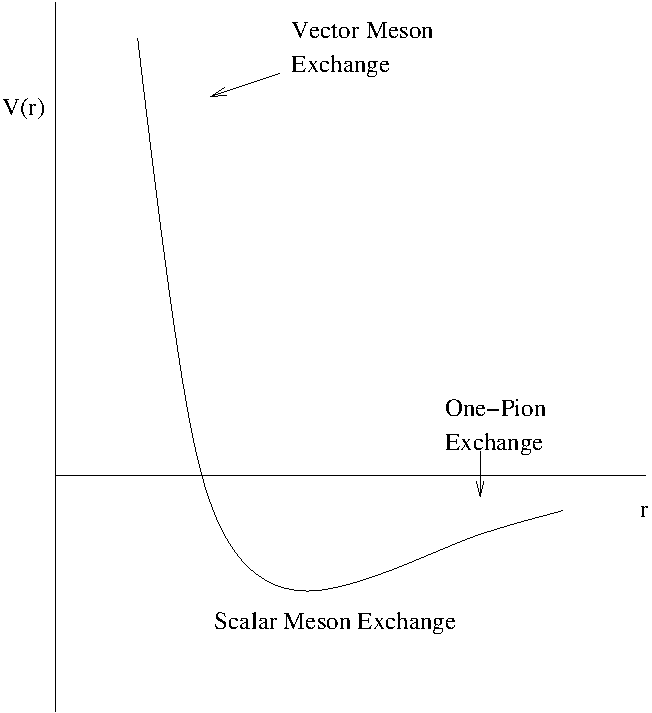
\includegraphics[scale=0.50]{nucleon-nucleon_pot}
\caption{The behavior of the nucleon-nucleon interaction}
\label{nucleon_pot}
\end{figure}

%Fig(\ref{nucleon_pot}) shows the behavior of the nucleon-nucleon interaction, it is repulsive at short distances. 


\section{Chiral Perturbation Theory}

The discovery of QCD and the understanding of effective field theory was a breakthrough for understanding the nucleon-nucleon potential.\\
 QCD is the 
theory of the strong interaction, where the quarks and gluons are treated as the degrees of freedom. 
The principles behind the theory are really simple and 
elegant, the interactions are derived by demanding that the Lagrangian is gauge invariant under SU(3). 
QCD is a non-Abelian field theory which is a consequence of 
the discovery of the three quantum numbers of color. The underlying gauge group is the SU(3) group. QCD is also known for "asymptotic freedom", the force
is weak at short distances but strong, at long distances or at low energies. The consequences of the asymptotic freedom is that the quarks are confined 
into "colorless" objects, called hadrons, and that perturbation theory in the low energy regime is strictly forbidden. As noted earlier nuclear physics 
is in this limit, and diffiulties arise when treating quarks and gluons in the nuclear force. 
The solution is to identify the relevant degrees of freedom, which in the nuclear case are the nucleons, we treat the nucleons as "elementary" particles 
and not a composite of quarks. When identifying the nucleons as the degrees of freedom we have to take in consideration the properties of the quarks,
they will be considered, but hidden in the coupling constants.\\

When constructing an effective field theory from QCD, all the symmetries 
of the Lagrangian should be manifest in the effective Lagrangian. In the case
of QCD, the Lagrangian is invariant under SU(3) transformation. \\
In the limit where the quark masses are zero, the chiral limit, the 
Lagrangian may be separated into a Lagrangian of left and right handed 
fields. The Lagrangian is invariant under left and right handed SU(3) 
transformations in the chiral limit.

We know that the quarks are not massless, but it is not a bad approximation
in the nuclear scale since $m_{u,d,s} \ll m_N$, where $u,d,s$ denotes the 
up, down and the strange quark, while $m_N$ stands for the nucleon mass. 
The remarkable theorem by Emma Noether states that for each symmetry of
the Lagrangian there exists a conserved current. In the case of chiral 
invariance the conserved currents are the left handed and the right handed 
ones. However these two currents can combine to a vector current 
$J^{\mu,b}_V$  and an axial current $J^{\mu , b}_A$. Where 

\be
\begin{split}
& J^{\mu, b}_V=R^{\mu, b} + L^{\mu,b }=\overline q \gamma^\mu \frac{\lambda^b}{2}q \\
& J^{\mu,b}_A=R^{\mu, b} - L^{\mu,b }=\overline q \gamma^\mu \gamma_5 \frac{\lambda^b}{2}q \\
\end{split}
\ee

For each current there is a corresponding charge, Q, which is a generator of $SU(3)_V\times SU(3)_A$, that is conserved.

The conserved charges will in this case be

\be
\begin{split}
& Q^b_V=\int d^3xJ^{0,b} \\
& Q^b_A=\int d^3xJ^{0,b}_A
\end{split}
\ee
 
When a mass term for the quarks are included in the Lagrangian, the symmetry
will break down, let us look at the QCD Lagrangian

\be
\mathcal L_{QCD}=\overline q(i\gamma^\mu D_\mu - M)q -\frac{1}{4}
G_{\mu \nu}^aG^{\mu \nu,a}.
\ee

By introducing explicitly the symmetry breaking mass term the currents will generally not be conserved, their divergences will satisfy

\be
\begin{split}
& \partial_\mu J^{\mu,a}_V=i\overline q[M,\frac{\lambda^a}{2}]q\\
& \partial_\mu J^{\mu,a}_A=i\overline q\{\frac{\lambda^a}{2},M\}\gamma_5 q.
\end{split}
\ee

For equal quark masses, the vector currents are conserved since all matrices commute with a multiple of the identity matrix. The axial currents are not
conserved. The symmetry breaks down to $SU(3)_V,$ in the case where the quarks have equal mass.\\

If the symmetry is spontaneously broken, the ground state is not invariant under a certain symmetry, the theory will be enriched by new particles, called
goldstone bosons. These particles will be massless and have the same quantum numbers as the generators that break the symmetry \cite{peskin}.\\
There are reasons to believe that the ground state is not annihilated by the generators of the axial symmetry. If there were an exact axial symmetry we 
would expect the existence of a degenerate hadron multiplet of opposite parity \cite{scherer2005}. For each hadron there should exist a hadron of opposite
parity. These multiplets are not observed. There exist a multiplet of particles in different isospin charges, the $\rho$ meson comes in three charge 
states, $\rho^\pm$ and $\rho^0$ which is equivalent to three isospin states. The $SU(3)_V$ is still a valid symmetry, but the $SU(3)_A$ is broken. 
As said earlier for each broken symmetry we will expect a massless goldstone boson. It is here the problem comes in, the standard
model doesn't account for any extra massless particles. This dilemma is solved by using the fact that the quarks are not massless, this implies that
the goldstone bosons acquire a small effective mass. The goldstone bosons are then identified as the pions, kaons and the $\eta$ particle, which have
the same quantum numbers as the broken generators. 
These goldstone bosons are then interpreted as the mediators in the nuclear interactions.

  


\section{$V_{low-k}$}

During the search for convergence of the two particle interaction diagrams in the laboratory system, I used $V_{low-k}$ to renormalize the 
nucleon-nucleon interaction. The method separates the Hilbert space in a low momentum part and a high momentum part \cite{bogner2003}. This is done by 
introducing a momentum cutoff in the momentum space, where all states with momenta higher than the cutoff belongs to the high momentum space.

As explained above, the nuclear potential is non perturbative in the nuclear limit, at high energies, or short distances the nucleon-nucleon interaction
becomes highly repulsive. By renormalizing the potential the repulsive and the non perturbative part of it "get swept under the carpet" as Zee in ref. \cite{nutshell} says it.% The astute reader 
%may wonder whether we loose to much physics by doing it, wouldn't much of the physics the potential explains be lost. The answer is that they are not 
%lost but hidden in the coupling constants that appear. 
There are many ways to renormalize the potential , or to get "rid off" the high momentum part, all of them, must have one thing in common. The renormalized
potential should give an accurate description of the low energy nucleon-nucleon scattering data. %In this case it is $V_{low-k}$ that is used.  

%The nucleon-nucleon interaction has to be treated perturbatively when computing a twobody perturbation diagram. 
The cut off in $V_{low-k}$ is done on the momentum. 
The cut off is based on two steps \cite{gamow}. 
Diagonalization of the momentum space for the relative momentum. The transformation of $k \in [0, \infty)$ to $k \in [0, \Lambda ]$.
A typical value of $\Lambda$ is approximately $2 fm^{-1},$ the renormalized potential, $V_{low-k}$, is dependent on the cutoff.

For deriving the effective potential we first have to consider the full many body system described by Schr\" odinger's equation

\be
H\ket{\Psi}=E\ket{\Psi}.
\ee

The Hamiltonian is separated in an unperturbed part and a perturbed part

\be
H=H_0+H_I.
\ee

Where $H_I$ denotes the perturbed Hamiltonian and describes the interaction part. 
The first part of constructing an effective Hamiltonian, is to define two projector operators that projects onto the low energy state. Usually the 
projector operator that projects onto the low energy state is symbolized with $P$ and the complement is denoted by $Q$. 
The projection operators satisfy the properties

\be
\begin{split}
& P^2=P\\
& Q^2=Q\\
& P+Q=1\\
& PQ=QP=0\\
& [H_0,P]=[H_0,Q]=0\\
& QH_0P=PH_0Q=0.
\end{split}
\ee

By using the projection operators the Hamiltonian may be written as 

\be
H=(P+Q)H(P+Q)=PHP+PHQ+QHP+QHQ
\ee

The Schr\" odinger equation can then be written in a matrix form 

\be
\begin{pmatrix}
PHP & PHQ\\
QHP &QHQ
\end{pmatrix}
\begin{pmatrix}
P\ket{\Psi}\\
Q\ket{\Psi}
\end{pmatrix}
= E
\begin{pmatrix}
P\ket{\Psi}\\
Q\ket{\Psi}
\end{pmatrix}.
\label{effh}
\ee


There exists two main methods for  solving the effective Hamiltonian, the first is the Bloch-Horowitz \cite{bloch58},\cite{blochhoro} where the effective Hamiltonian turns out to be 
dependent on the exact energy eigenvalue one is solving for, and the Lee-Suzuki method \cite{suzlee},\cite{leesuz}. The two methods are thoroughly 
compared in \cite{jennings-2005-72}.
Both of the methods want the effective Hamiltonian to be of the form 

\be
H_{eff}=PHP
\ee

The solution of the Bloch-Horowitz effective Hamiltonian is

\be
\mathcal H^{BH}_{eff} =P( H +H\frac{1}{E-QHQ}H)P
\ee

The corresponding eigenvalue problem 

\be
P( H +H\frac{1}{E-QHQ}H)PP\ket{\Psi}=EP\ket{\Psi}
\ee

has to be solved by a self consistent treatment. 

The Lee-Suzuki method avoids the difficulties with the energy eigenvalue in the effective Hamiltonian by constructing a similarity transformation of 
the Hamiltonian in Eq. \eqref{effh} to the structure 

\be
H^{LS}=
\begin{pmatrix}
P\mathcal H P & P \mathcal H Q\\
0 & Q\mathcal H Q
\end{pmatrix}
=X^{-1}HX
\ee

The condition for $P\mathcal H P$ to be the P space effective Hamiltonian is that

\be
QX^{-1}HXP=0
\label{waveop}
\ee 

The choice of $X$ is crucial, different choice of X leads to different many body theory, Lee and Suzuki \cite{suzlee} made the ansatz of 

\be
\begin{split}
& X=e^\omega\\
& \mathcal H = e^{-\omega}He^\omega.
\end{split}
\ee

Where $\omega$ is the so called wave operator it connects the $P$ and $Q$ space in the sense that it transform the state
$P\ket{\Psi}$ to the state $Q\ket{\Psi}.$ With the wave operator on the form $\omega=Q\omega P$ the condition \eqref{waveop} is satisfied. This will
also constrain the matrix $X$ by the following properties of the wave operator

\be
\begin{split}
& P\omega P=PQ\omega PP=0 \\
& Q\omega Q=QQ\omega PQ=0\\
& P \omega Q=PQ \omega QQ=0\\
& \omega ^2= Q\omega PQ\omega P=0
\label{waveopconstraint}
\end{split}
\ee

The expansion of X will then consist of just two terms

\be
X=e^\omega = 1 + \omega=1 + Q \omega P
\ee


The four parts of of the Hamiltonian matrix in \eqref{effh} will then be expressed as 

\be
\begin{split}
& P\mathcal H P=PHP + PH_IQ\omega P\\
& P\mathcal H Q = PH_IQ\\
& Q\mathcal H Q= QHQ - \omega PH_IQ\\
& Q\mathcal H P=QH_IP + QHQ\omega - \omega PHP -\omega PH_I Q\omega
\label{effectivepart}
\end{split}
\ee

With Eq. \eqref{waveopconstraint} and Eq. \eqref{effectivepart} we get an equation for the waveoperator.

\be
QH_IP+QHQ\omega -\omega PHP -\omega PH_IQ\omega = 0
\label{qhp0}
\ee

If we have a solution for $\omega$ it is then just to replace it for $\omega$ in our effective Hamiltonian

\be
H_{eff}= PHP + PH_IQ\omega P
\ee

By defining the $P$ space effective interaction operator

\be
V_{eff}=H_{eff}-PH_0P=PH_IP +PH_IQ\omega.
\ee

The $P$ space eigenvalue problem can be written as 

\be
H_{eff}\ket{\psi_\mu}=(PH_0P+V_{eff})\ket{\psi_\mu}=E_\mu \ket{\psi_\mu}
\ee

The wave operator can be solved in terms of the eigenvalue and eigenstates $E_\mu$ and $\ket{\psi_\mu}.$

\be
\omega(E_\mu)=\sum_{\mu=1}^d\frac{1}{E_\mu-QHQ}QH_IP\ket{\psi_\mu}\bra{\tilde{\psi}_\mu}.
\label{omega}
\ee

$\bra{\tilde{\psi}_\mu}$ is the bi orthogonal state corresponding to $\ket{\psi_\mu}.$ There are various methods to solve the non-linear equation for the
wave operator. For the two body problem the exact solutions for the eigenstates can be used, and the effective interaction can be calculated directly by 
using Eq. \eqref{omega}. For more complex applications the equation has to be solved iteratively.  
